% TODO rimuovere
%\section{Obbiettivi}

%sembra OK
\begin{frame}{Obbiettivi}
  \begin{columns}
    \begin{column}{.7\textwidth}
      \begin{itemize}%[<+->]
        \item \textbf{O1}: \alert{Estensione dell'Assurance Engine} per supportare il monitoraggio basato su \alert{Elasticsearch}
        
        \item \textbf{O2}: Implementazione di \alert{contratti} basati su \alert{\textit{evidence}} per eseguire \alert{valutazioni} di PNF 
  
        \item \textbf{O3}: Valutazione sperimentale delle \alert{performance del sistema} in un cluster Kubernetes
      \end{itemize}
    \end{column}

    \begin{column}{.2\textwidth}
      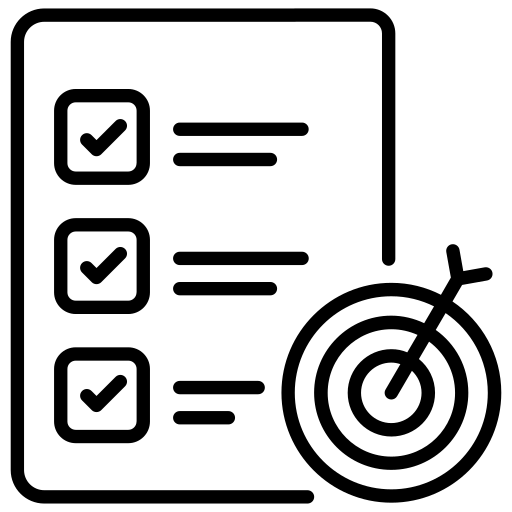
\includegraphics[scale=.16]{assets/icon/03obbiettivi_objectives.png}
    \end{column}

  \end{columns}
  
\end{frame}


	
